% sample: clutter rate=50, sample no. 008

The third case depicts the same scenario as (C2), however, with two additional targets that appear at unexpected locations. Figure \ref{fig:c3-results-overview} shows that the GM-PHD filter fails to estimate states of these two additional targets. On the right side of this figure, we see that there are no black circles for two lines on both the X axis, and the Y axis. The figures illustrating the change in metrics over different values of filter parameters is located in Appendix \ref{appendix:results-figures}.

\begin{figure*}
    \centering
    \begin{subfigure}[]{0.48\linewidth}
        \centering
        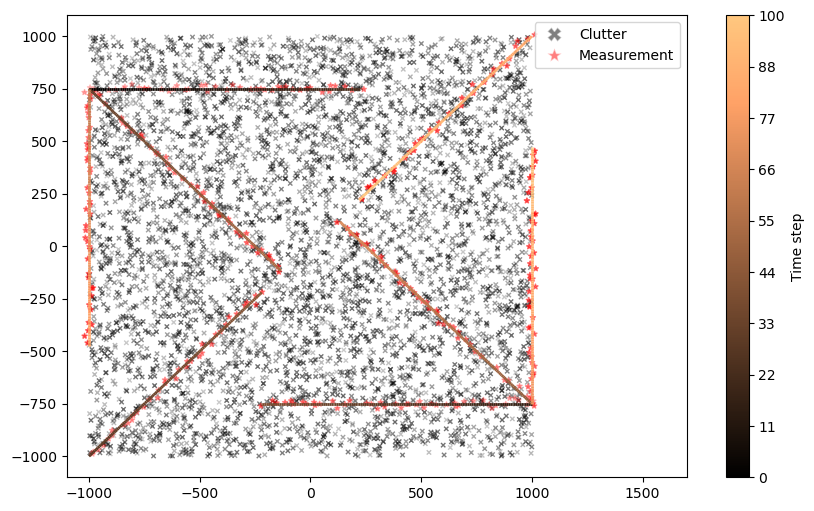
\includegraphics[width=\linewidth]{figures/c3-tracks-measurements.png}
    \end{subfigure}
    \hfill
    \begin{subfigure}[]{0.48\linewidth}
        \centering
        \begin{subfigure}[t]{\linewidth}
            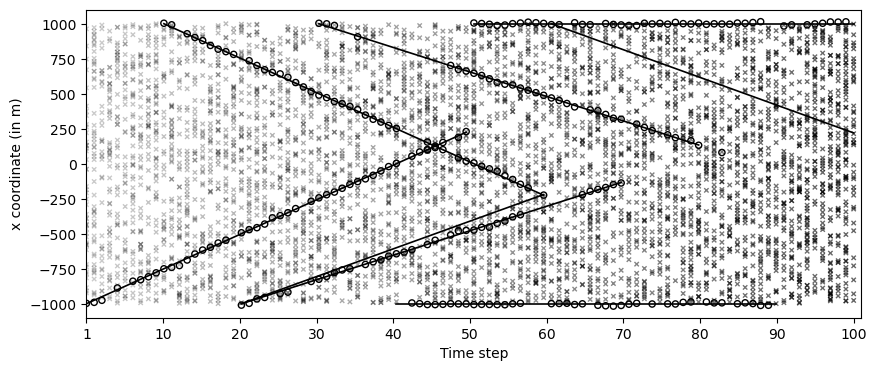
\includegraphics[width=\linewidth]{figures/c3-x-estimates.png}
        \end{subfigure}
        \vfill\par
        \begin{subfigure}[b]{\linewidth}
            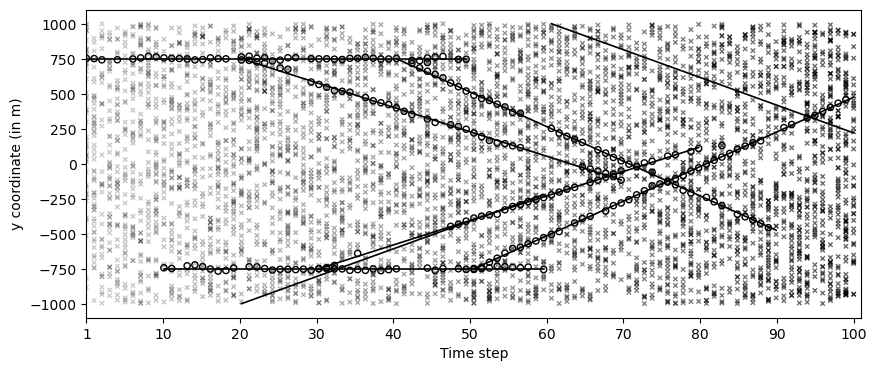
\includegraphics[width=\linewidth]{figures/c3-y-estimates.png}
        \end{subfigure}
    \end{subfigure}
  \caption[One sample of data and estimates for the (C3) scenario.]{One sample of data and estimates for the (C3) scenario. Left: True tracks of two objects (black to yellow) with clutter measurements (gray crosses) and received measurements (red stars) for a single Monte Carlo sample. Right: Change of both coordinates in time with noise measurements (red circles) and filter estimates (black circles) for the same Monte Carlo sample. Two targets were not detected by the filter, and no estimates were generated for them.}
  \label{fig:c3-results-overview}
\end{figure*}


If we look at Figure \ref{fig:c3-traj-post}, we will clearly see, that two targets starting from the bottom-left corner and the top-right corner were not detected by the filter. The track continuity problem persists. It should be noted, that for the demonstration purposes, we intentionally choose the sample where the track continuity problem is present and visible. Generally, the filter performs well, and the expected absolute error on the number of targets should be compared using the average value over all samples.

\begin{figure}
    \centering
    \begin{subfigure}[]{0.48\linewidth}
        \centering
        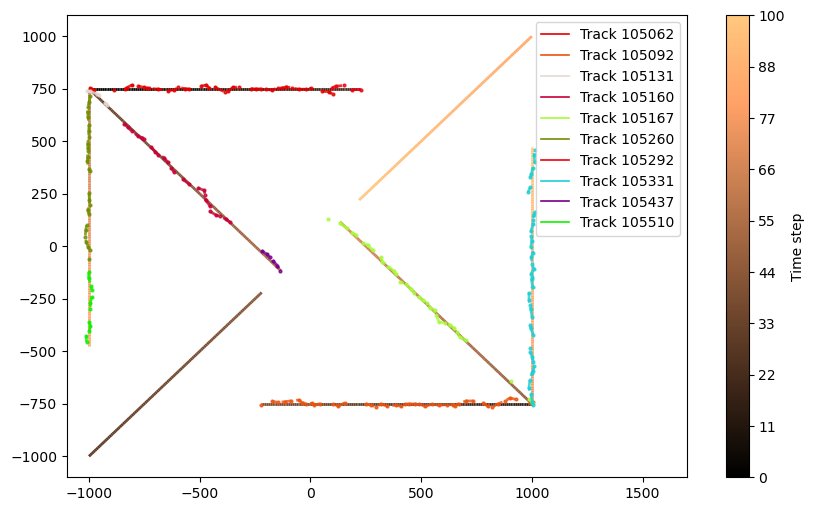
\includegraphics[width=\linewidth]{figures/c3-traj.png}
    \end{subfigure}
    \hfill
    \begin{subfigure}[]{0.48\linewidth}
        \centering
        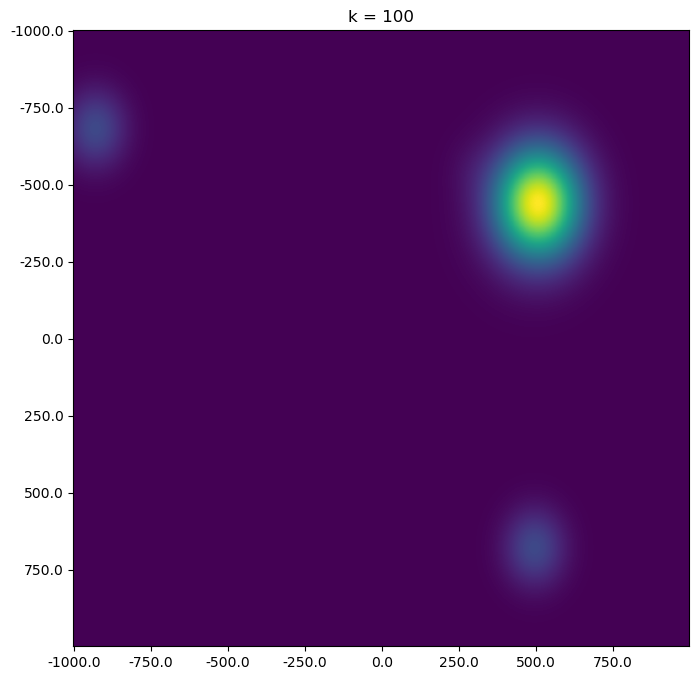
\includegraphics[width=\linewidth]{figures/c3-post.png}
    \end{subfigure}
  \caption[(C3). Trajectories estimations and the posterior intensity.]{Left: The visualization of trajectories estimates and the posterior distribution at time $k=100$. Two targets were not detected. Right: The posterior distribution at time step $k=100$. For visualization purposes, the covariance matrices of all Gaussian components were multiplied by the factor of $81$. The filter was run with default settings, i.e. $\lambda_{c} = 12.5 \times 10^{-6}$, $P_{D,k} = 0.98$, $P_{S,k} = 0.99$, $\tau = 10^{-5}$, and $U=4$.}
  \label{fig:c3-traj-post}
\end{figure}
